\begin{refsection}

\chapter{Ar--Ar and K--Ca}
\label{ch:ArArKCa-R}

\section{Ar--Ar}\label{sec:ArAr-R}

\texttt{IsoplotR} accommodates three Ar--Ar formats. See
Section~\ref{sec:ArAr} for details. The left hand side of the GUI
contains the usual input table, as well as two text boxes for the
J-factor and its standard error:

\noindent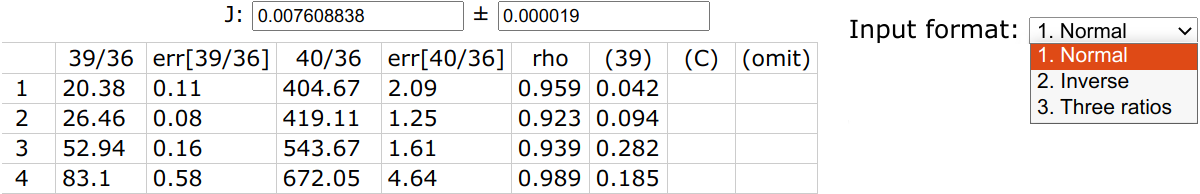
\includegraphics[width=\linewidth]{../figures/ArArInputTableFormats.png}\\

The input files for the CLI represent the same structure: they contain
both the J factor and the isotopic ratio data.

\begin{console}
ArAr <- read.data('ArAr1.csv',method='Ar-Ar',format=1)
\end{console}

The output of the \texttt{read.data()} function reflects the contents
of the input file. It returns a list with three items:

\begin{enumerate}
\item\texttt{format} stores the value of the eponymous input argument,
\item\texttt{J} is a two-element vector with the J-factor and its standard error,
\item\texttt{x} contains the isotopic ratio data.
\end{enumerate}
  
\noindent\begin{minipage}[t]{.15\linewidth}
\strut\vspace*{-\baselineskip}\newline
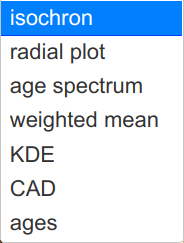
\includegraphics[width=\linewidth]{../figures/ArArPlotdevices.png}\\
\end{minipage}
\begin{minipage}[t]{.85\textwidth}
  Ar--Ar data can be visualised on six different plot devices.
  Additionally, the single aliquot age estimates can also be reported
  in a downloadable data table.
\end{minipage}

The default atmospheric \textsuperscript{40}Ar/\textsuperscript{36}Ar
ratio is given by \citet{lee2006}, and the \textsuperscript{40}K decay
constant by \citet{renne2011}. These values can be changed here:\\

\noindent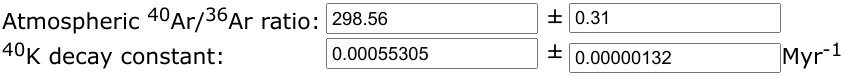
\includegraphics[width=.7\linewidth]{../figures/ArArLambda.png}

\begin{script}
# use the atmospheric ratio from Nier (1950):
settings('iratio','Ar40Ar36',295.5,0.5)
\end{script}

\section{K--Ca}\label{sec:KCa-R}

\noindent\begin{minipage}[t]{.3\linewidth}
\strut\vspace*{-\baselineskip}\newline
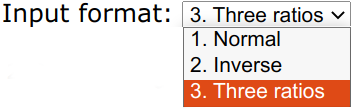
\includegraphics[width=\linewidth]{../figures/PbPbFormats.png}
\end{minipage}
\noindent\begin{minipage}[t]{.15\linewidth}
\strut\vspace*{-\baselineskip}\newline
\includegraphics[width=\linewidth]{../figures/PbPbPlotdevices.png}
\end{minipage}
\begin{minipage}[t]{.55\textwidth}
  \texttt{IsoplotR} accommodates three K--Ca formats (see
  Section~\ref{sec:K-Ca} for details), which can be analysed by the
  same methods as the Ar--Ar method with the exception of the age
  spectra function.
\end{minipage}

\begin{console}
KCa <- read.data('KCa3.csv',method='K-Ca',format=3)
\end{console}

\noindent returns a list with items \texttt{format} and \texttt{x}
containing the input format and isotopic ratio data, respectively.\\

\noindent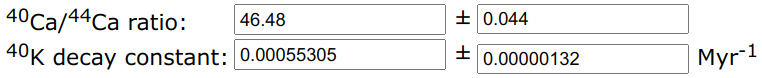
\includegraphics[width=.7\linewidth]{../figures/KCaLambda.png}\\

\noindent The default value for the inherited Ca component is given by
\citet{moore1972}. This option is hidden from the \texttt{isochron}
function. The default K decay constant is the same as for the Ar--Ar
method \citep{renne2011}.

\begin{script}
# use the Steiger and Jaeger (1977) decay constant with zero uncertainty
settings('lambda','K40',5.543e-4,0)
\end{script}

\section{Isochrons}\label{sec:ArAr-isochrons-R}

\begin{enumerate}

\item \texttt{IsoplotR} offers the same three options to deal with the
  scatter of the data around the best-fit isochron line as the generic
  regression function of Section~\ref{sec:OtherRegression} and the
  Pb--Pb isochron function (Section~\ref{sec:PbPb-isochrons-R}).

\noindent\begin{minipage}[t]{.45\linewidth}
\strut\vspace*{-\baselineskip}\newline
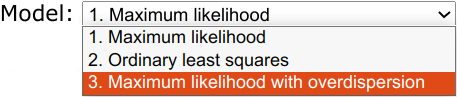
\includegraphics[width=\linewidth]{../figures/ArArIsochronModels.png}
\end{minipage}
\begin{minipage}[t]{.55\linewidth}
  These three models represent three different ways to capture any
  excess dispersion of the data relative to the nominal uncertainties
  (Figure~\ref{fig:isochronMSWD}).
\end{minipage}

\begin{console}
isochron(ArAr,model=3)
\end{console}

\noindent\begin{minipage}[t]{.45\linewidth}
\strut\vspace*{-\baselineskip}\newline
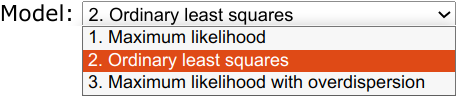
\includegraphics[width=\linewidth]{../figures/KCaIsochronModels.png}
\end{minipage}
\begin{minipage}[t]{.55\linewidth}
  The same three models are available for K--Ca data as well.
\end{minipage}

\begin{console}
isochron(KCa,model=2)
\end{console}

\item \noindent\begin{minipage}[t]{.22\linewidth}
\strut\vspace*{-\baselineskip}\newline

\includegraphics[width=\linewidth]{../figures/ArArisochronInverse.png}
\end{minipage}
\begin{minipage}[t]{.78\linewidth}
Data can be fitted using conventional
(\textsuperscript{40}Ar/\textsuperscript{36}Ar
vs. \textsuperscript{39}Ar/\textsuperscript{36}Ar) or inverse
(\textsuperscript{36}Ar/\textsuperscript{40}Ar
vs. \textsuperscript{39}Ar/\textsuperscript{40}Ar) isochrons
(Section~\ref{sec:inverseIsochrons}).
\end{minipage}

\begin{console}
isochron(ArAr,inverse=FALSE)
\end{console}

\noindent\begin{minipage}[t]{.22\linewidth}
\strut\vspace*{-\baselineskip}\newline

\includegraphics[width=\linewidth]{../figures/PbPbisochronInverse.png}
\end{minipage}
\begin{minipage}[t]{.78\linewidth}
For the K--Ca method, conventional isochrons plot
\textsuperscript{40}Ca/\textsuperscript{44}Ca against
\textsuperscript{40}K/\textsuperscript{44}Ca, and inverse isochrons
plot \textsuperscript{44}Ca/\textsuperscript{40}Ca against
\textsuperscript{40}K/\textsuperscript{40}Ca.
\end{minipage}

\begin{console}
isochron(KCa,inverse=TRUE)
\end{console}

\item The appearance and numerical behaviour of Ar--Ar and K--Ca
  isochrons can be modified using the same options as the Pb--Pb
  isochrons of Section~\ref{sec:PbPb-isochrons-R}, and the general
  regression of Section~\ref{sec:OtherRegression}.

\noindent\begin{minipage}[t]{.45\linewidth}
\strut\vspace*{-\baselineskip}\newline
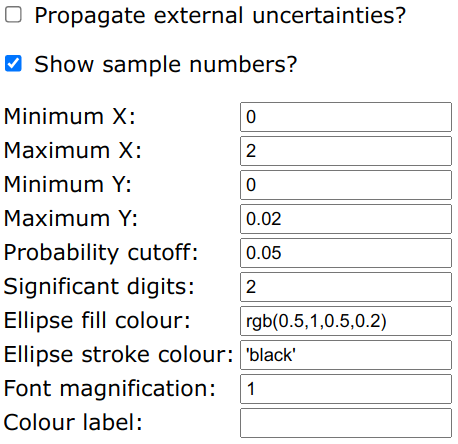
\includegraphics[width=\linewidth]{../figures/KCaIsochronOtherOptions.png}
\end{minipage}
\begin{minipage}[t]{.55\linewidth}
Tick the checkbox to propagate decay constant uncertainties
(\texttt{exterr}) and label the error ellipses with the row numbers of
the input data (\texttt{show.numbers}), use the textboxes to set the
axis limits (\texttt{xlim} and \texttt{ylim}), significance level
(\texttt{alpha}) and significant digits (\texttt{sigdig}), as well as
the fill and stroke colour of the error ellipses
(\texttt{ellipse.fill} and \texttt{ellipse.stroke}), font size
(\texttt{cex}) and colour legend (\texttt{levels} and
\texttt{clabel}).
\end{minipage}

\begin{script}
isochron(KCa,inverse=TRUE,exterr=FALSE,show.numbers=TRUE,
         xlim=c(0,2),ylim=c(0,0.02),ellipse.fill=rgb(0.5,1,0.5,0.2))
\end{script}
  
\end{enumerate}

\section{Ages}\label{sec:ArArKCaAges}

Like the Pb--Pb and Th--Pb methods of Chapter~\ref{ch:ThPbPb-R}, also
the K--Ca method is usually applied to cogenetic aliquots for isochron
regression. However the Ar--Ar method is also commonly applied to
detrital grains, which may exhibit a wide range of true ages.  For
both the Ar--Ar and K--Ca methods, \texttt{IsoplotR} produces data
tables of the single aliquot age estimates, which can be further
analysed and displayed as age spectra, and radial, weighted mean, KDE
and CAD plots.

The atmospheric argon correction for the Ar--Ar ages can be specified
in one of two ways:\\

\noindent\begin{minipage}[t]{.5\linewidth}
\strut\vspace*{-\baselineskip}\newline

\includegraphics[width=\linewidth]{../figures/ArAri2i.png}
\end{minipage}
\begin{minipage}[t]{.5\linewidth}
Ticking this box uses the y-intercept of an isochron fit through all
the Ar data as an initial
\textsuperscript{40}Ar/\textsuperscript{36}Ar-ratio for the age
calculations. Unticking it uses nominal atmospheric ratio of
Section~\ref{sec:ArAr-R}.
\end{minipage}

\begin{script}
# i2i stands for 'intercept to initial'
age(ArAr,i2i=TRUE) 
\end{script}

\noindent\begin{minipage}[t]{.5\linewidth}
\strut\vspace*{-\baselineskip}\newline

\includegraphics[width=\linewidth]{../figures/KCai2i.png}
\end{minipage}
\begin{minipage}[t]{.5\linewidth}
Similarly, for the K--Ca method, the inherited
\textsuperscript{40}Ca-component can be removed by projection along
the inverse isochron.
\end{minipage}

\begin{console}
age(KCa,i2i=TRUE)
\end{console}

\noindent\begin{minipage}[t]{.55\linewidth}
\strut\vspace*{-\baselineskip}\newline
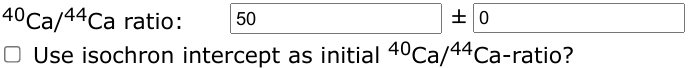
\includegraphics[width=\linewidth]{../figures/KCaNominalInitials.png}
\end{minipage}
\begin{minipage}[t]{.45\linewidth}
Alternatively, the initial \textsuperscript{40}Ca can be removed by
means of a nominal
\textsuperscript{40}Ca/\textsuperscript{44}Ca-correction.
\end{minipage}

\begin{script}
settings('iratio','Ca40Ca44',50,0)
age(KCa,i2i=FALSE)
\end{script}

\noindent\begin{minipage}[t]{.5\linewidth}
\strut\vspace*{-\baselineskip}\newline

\includegraphics[width=\linewidth]{../figures/ArArProjerr.png}
\end{minipage}
\begin{minipage}[t]{.5\linewidth}
  The analytical error of the initial \textsuperscript{40}Ar- or
  \textsuperscript{40}Ca-correction can be added to the age
  uncertainty.
\end{minipage}

This part-systematic, part-random uncertainty may cause strong error
correlations between the different aliquots of a single sample. But
when considering each aliquot in isolation (for example, the
\texttt{i=2}\textsuperscript{th} aliquot), the full error propagation
with decay constant uncertainties (\texttt{exterr}) and initial
daughter correction uncertainty (\texttt{projerr}) does provide the
most faithful estimate of the true age uncertainty:

\begin{script}
age(ArAr,i2i=TRUE,projerr=TRUE,i=2)
\end{script}

\section{Ar--Ar age spectra}\label{sec:ArArAgeSpectra}

There are just two minor differences between the Ar--Ar age spectrum
function and the generic age spectrum function of
Section~\ref{sec:OtherAgeSpectra}. First, an atmospheric argon
correction can be made to each aliquot in exactly the same way as
described in Section~\ref{sec:ArArKCaAges}, either using a nominal
value or the isochron intercept:

\begin{console}
agespectrum(ArAr,plateau=TRUE,i2i=FALSE)
\end{console}

\noindent\begin{minipage}[t]{.35\linewidth}
\strut\vspace*{-\baselineskip}\newline

\includegraphics[width=\linewidth]{../figures/ArArExterr.png}
\end{minipage}
\begin{minipage}[t]{.65\linewidth}
Second, the \textsuperscript{40}K decay constant uncertainty can be
propagated into the plateau age.
\end{minipage}

\begin{console}
agespectrum(ArAr,plateau=TRUE,exterr=TRUE)
\end{console}

The remaining options are the same as the generic age spectrum
function:\\

\noindent\begin{minipage}[t]{.4\linewidth}
\strut\vspace*{-\baselineskip}\newline
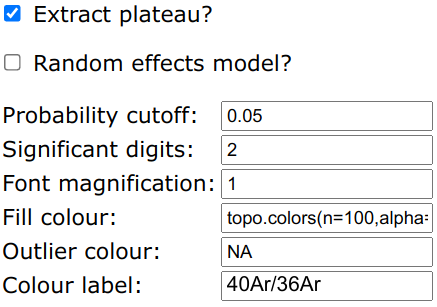
\includegraphics[width=\linewidth]{../figures/ArArAgeSpectrumOtherOptions.png}\\
\end{minipage}
\begin{minipage}[t]{.6\linewidth}
  If requested, the plateau age can be computed either using the
  ordinary weighted mean algorithm of Equation~\ref{eq:wtdmean}, or
  the random effects model of Equation~\ref{eq:wtdmean-model-3}.  The
  rectangular segments of the age spectrum can be coloured based on
  any additional parameter. Here a reversed(rainbow) colour ramp is
  used for aliquots that belong to the age plateau, whereas segments
  that do not belong to the plateau are left empty.
\end{minipage}

At the CLI, the \textsuperscript{40}Ar/\textsuperscript{36}Ar-ratio
that forms the basis of the colour scale can be extracted from the
\texttt{ArAr} data object, and the colour label can be typeset using
an \texttt{R}-expression for the
\textsuperscript{40}Ar/\textsuperscript{36}Ar ratio that includes
superscripts:

\begin{script}
agespectrum(ArAr,levels=ArAr$x[,'Ar40Ar36'],plateau=TRUE,
            plateau.col=rev(rainbow(n=100,alpha=0.5)),
            exterr=TRUE,i2i=FALSE,random.effects=FALSE,
            clabel=expression(''^40*'Ar/'^36*'Ar'))
\end{script}
  
\section{Radial, weighted mean, KDE and CAD plots}
\label{sec:ArArKCaOtherPlots}

The settings for the radial, weighted mean, KDE and CAD plots combine
the generic settings for those graphical devices
(Sections~\ref{sec:OtherRadial}--\ref{sec:OtherCAD}) with the settings
for the age calculator.\\

\noindent\begin{minipage}[t]{.5\linewidth}
\strut\vspace*{-\baselineskip}\newline
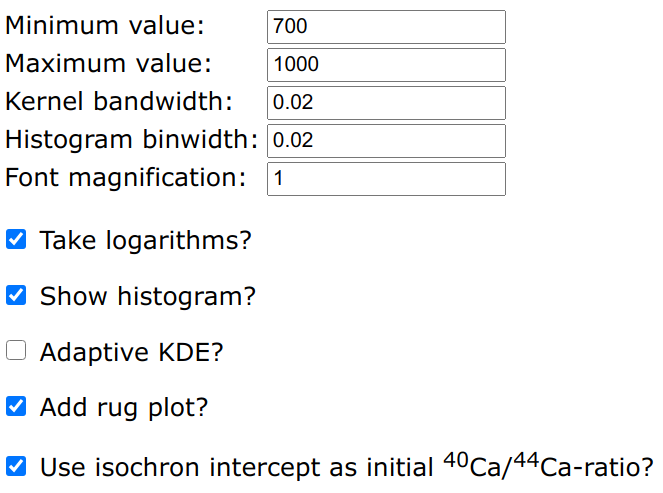
\includegraphics[width=\linewidth]{../figures/KCaKDE.png}
\end{minipage}
\begin{minipage}[t]{.5\linewidth}
  For example, here are shown the GUI settings for a KDE plot of the
  \texttt{KCa} dataset, which is plotted on a logarithmic scale that
  stretches from 700 to 1000~Ma and uses a fixed kernel bandwidth and
  binwidth of 2\%.
\end{minipage}

\begin{script}
kde(KCa,log=TRUE,from=700,to=1000,bw=0.02,
    binwidth=0.02,adaptive=FALSE,i2i=TRUE)
\end{script}

Similarly, the weighted mean, radial plot and CAD functions work
exactly like the generic versions of Chapter~\ref{ch:generic-R}, with
the only difference being the inherited daughter correction, and the
ability to propagate external uncertainties.\\

\noindent CLI examples:

\begin{enumerate}

\item A radial plot on a logarithmic scale that ranges 60 to 64~Ma and
  is centred at 61~Ma, with samples coloured according to their
  measured \textsuperscript{40}Ar/\textsuperscript{36}Ar-ratio:

\begin{script}
radialplot(ArAr,from=60,to=64,z0=61,levels=ArAr$x[,'Ar40Ar36'],
           clabel=expression(''^40*'Ar/'^36*'Ar'))
\end{script}

\item The weighted mean using a nominal atmospheric argon correction
  with \citet{nier1950}'s
  \textsuperscript{40}Ar/\textsuperscript{36}Ar value; applying the
  random effects model and plotting the ranked ages:
  
\begin{script}
settings('iratio','Ar40Ar36',295.5,0.5)
weightedmean(ArAr,i2i=FALSE,random.effects=TRUE,ranked=TRUE)
\end{script}

\item A CAD without vertical lines:

\begin{console}
cad(KCa,verticals=FALSE)
\end{console}
  
\end{enumerate}

\printbibliography[heading=subbibliography]

\end{refsection}
